% =======================================================
% 5. RESOCONTO ATTIVITA' DI VERIFICA
% =======================================================
\section{Resoconto Attività di Verifica}
In questa sezione vengono riportati i risultati delle attività di verifica condotte fino alla fase di Product Baseline\textsubscript{G} (PB), a integrazione di quanto già rendicontato in fase di RTB. L'obiettivo è fornire una panoramica oggettiva del livello di qualità raggiunto.

\subsection{Verifica documentazione}
La verifica della documentazione (Analisi dei Requisiti, Norme di Progetto, Piano di Progetto, Verbali e Glossario) è avvenuta tramite revisione manuale incrociata. Il Verificatore\textsubscript{G} ha controllato la coerenza dei contenuti, l'assenza di errori grammaticali e il rispetto degli standard di formattazione definiti nelle \link{https://synergo-unit-unipd.github.io/Second-Brain/docs/PB/doc_gestionali/doc_interni/norme_di_progetto/norme_di_progetto.pdf}{Norme di Progetto}.
\\ \\
Tutti i documenti pubblicati hanno superato il controllo di qualità, raggiungendo un indice di leggibilità conforme ai parametri accettabili.

\subsection{Verifica codice}
In fase PB la verifica del codice è pienamente operativa: test automatizzati eseguiti con pytest per il backend e vitest per il frontend (comprensivi, per quest'ultimo, sia dei Test di Unità sia dei Test di Sistema di cui alla Sezione 4), integrati da controlli di qualità statica tramite eslint, prettier, ruff e mypy. L'intera suite è richiamata dal comando \texttt{make ci} ed eseguita automaticamente in CI a ogni Pull Request, con verifica delle soglie di copertura (Sezione 4.2).

\subsection{Copertura test}
La copertura è duplice. Da un lato, tracciabilità: il 100\% degli UC obbligatori individuati è coperto da almeno un Test di Sistema con stato Superato (Tabella~\ref{tab:test-sistema}); i soli UC non coperti (UC150--155) corrispondono a requisiti esplicitamente opzionali, non implementati per scelta. Dall'altro, copertura di codice: 95\% sul backend (soglia CI 90\%) e 89,75\% linee / 88,51\% statement / 89,72\% funzioni / 83,76\% branch sul frontend (soglie CI rispettivamente 85\%/83\%/78\%/78\%), entrambe verificate da \texttt{make coverage}.

\subsection{Esiti test}
La suite completa conta 511 casi automatizzati (63 di unità e integrazione sul backend via pytest, 447 tra unità e sistema sul frontend via vitest, 1 di deployment via script), tutti eseguiti con esito positivo: \textbf{511/511 superati}. La copertura di codice (Sezione 4.2) e la tracciabilità UC\,$\leftrightarrow$\,Test di Sistema sono verificate e documentate nella Specifica dei Test (Sezione 4).

\newpage
% =======================================================
% 6. VALUTAZIONI PER IL MIGLIORAMENTO
% =======================================================
\section{Valutazioni per il Miglioramento}
Il gruppo Synergo Unit adotta il metodo \textbf{PDCA} (Plan-Do-Check-Act) per garantire il miglioramento continuo dei processi.

\subsection{Retrospettive}
Al termine di ogni Sprint, il gruppo si riunisce per analizzare cosa ha funzionato e cosa può essere ottimizzato. Durante la RTB, è emersa la necessità di automatizzare maggiormente la compilazione di alcune tabelle LaTeX per ridurre il tempo di verifica manuale.

\subsection{Azioni correttive}
A fronte di anomalie rilevate dalle metriche o durante le revisioni, sono state stabilite le seguenti contromisure:

\begin{table}[H]
    \centering
    \renewcommand{\arraystretch}{1.3}
    \begin{tabularx}{\textwidth}{|p{6cm}|p{6.5cm}|X|}
        \hline
        \rowcolor{primarycolor!10}
        \textbf{Problema Rilevato} & \textbf{Contromisura Adottata} & \textbf{Rischio correlato} \\
        \hline
        Difficoltà iniziale nella gestione della sintassi LaTeX complessa. & Creazione di un repository di template\textsubscript{G} condivisi per tabelle e strutture ricorrenti. & RT1 \\
        \hline
        Incoerenza nella numerazione dei Casi d'Uso (UC) tra diversi documenti. & Revisione centralizzata dell'Analisi dei Requisiti e allineamento immediato dei test. & RR1, RO5 \\
        \hline
        Frequenti conflitti durante l'unione del codice sorgente (merge conflicts). & Utilizzo sistematico di un repository GitHub e adozione di un workflow basato su branch\textsubscript{G} per isolare le funzionalità. & RT4 \\
        \hline
        Difficoltà nel tracciamento puntuale delle attività (task) e delle ore spese dai singoli membri. & Utilizzo di GitHub Projects e GitHub Issues per l'assegnazione dei compiti e il monitoraggio dello stato di avanzamento (ToDo, In Progress, In Review, Done). & RO3 \\
        \hline
        Eccessivo carico burocratico e rischio di errore umano nella creazione manuale dei task e nella raccolta dati. & Automazione del processo tramite un form dedicato per la generazione automatica delle Issue. I dati vengono centralizzati in un foglio di calcolo\textsubscript{G} per la generazione automatica della rendicontazione e del cruscotto. & RO6, RO7 \\
        \hline
    \end{tabularx}
    \caption{Storico delle azioni correttive}
\end{table}

\subsection{Problemi aperti}
Nessuno. Tutti i livelli di test previsti (unità, integrazione, sistema) sono implementati, integrati in CI ed eseguiti con esito interamente positivo (Sezione 4); il framework di testing per l'integrazione con le API LLM, questione aperta in fase RTB, è stato adottato stabilmente (pytest per il backend, vitest per il frontend) e non presenta criticità residue.

\newpage
% =======================================================
% 7. CRUSCOTTO DELLE METRICHE
% =======================================================
\section{Cruscotto delle Metriche}
In questa sezione sono riassunti i valori ottenuti dalle metriche durante l'ultimo Sprint della fase PB.

\subsection{Stato attuale qualità di processo}
\begin{table}[H]
    \centering
    \renewcommand{\arraystretch}{1.3}
    \begin{tabularx}{\textwidth}{|l|X|c|c|}
        \hline
        \rowcolor{primarycolor!10}
        \textbf{Codice} & \textbf{Nome Metrica} & \textbf{Valore Rilevato} & \textbf{Esito} \\
        \hline
        MPC01 & Schedule Performance Index & 1.00 & Ottimale \\
        \hline
        MPC02 & Cost Performance Index & 0.99 & Accettabile \\
        \hline
        MPC03 & Requirements Stability Index & 88,46\% & Accettabile \\
        \hline
        MPC04 & Time Efficiency & 100\% & Ottimale \\
        \hline
        MPC05 & Task Completion Rate & 100\% & Ottimale \\
        \hline
        MPC06 & PR Resolution Time & 2 giorni & Accettabile \\
        \hline
        MPC07 & Review Coverage & 100\% & Ottimale \\
        \hline
        MPC08 & Quality Metrics Compliance Rate & 100\% & Ottimale \\
        \hline
    \end{tabularx}
    \caption{Riepilogo Qualità di Processo}
\end{table}

\subsection{Stato attuale qualità di prodotto}
\begin{table}[H]
    \centering
    \renewcommand{\arraystretch}{1.3}
    \begin{tabularx}{\textwidth}{|l|X|c|c|}
        \hline
        \rowcolor{primarycolor!10}
        \textbf{Codice} & \textbf{Nome Metrica} & \textbf{Valore Rilevato} & \textbf{Esito} \\
        \hline
        MPD01 & Soddisfacimento Requisiti Obbligatori & 100\% & Ottimale \\
        \hline
        MPD02 & Comment Density & 15,11\% & Accettabile \\
        \hline
        MPD03 & Browser Compatibility & 3 & Accettabile \\
        \hline
        MPD04 & Errori Ortografici (per pagina) & 0 & Ottimale \\
        \hline
        MPD05 & Complessità Ciclomatica & 2,64 & Ottimale \\
        \hline
        MPD06 & Tempo di Caricamento Iniziale & 2,9 s & Soddisfatto \\
        \hline
        MPD07 & Indice di Gulpease (Media Documenti) & 51,90 & Accettabile \\
        \hline
    \end{tabularx}
    \caption{Riepilogo Qualità di Prodotto}
\end{table}


\subsection{Grafici e dashboard}
L'andamento storico delle metriche viene monitorato tramite grafici temporali per evidenziare eventuali trend negativi.

\subsubsection{Trend di Progetto}
 \begin{figure}[H]
	    \centering
	    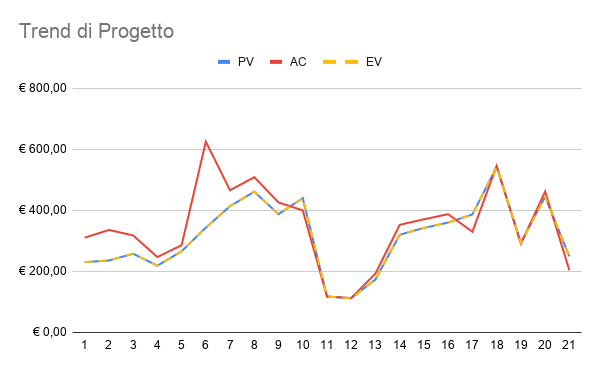
\includegraphics[width=0.8\textwidth]{grafici/trend.png}
	    \caption{Andamento PV\textsubscript{G}, AC\textsubscript{G}, EV\textsubscript{G}}
	 \end{figure}

Il grafico riporta l'andamento cumulato, sprint dopo sprint, del Planned Value\textsubscript{G} (PV), dell'Actual Cost\textsubscript{G} (AC) e dell'Earned Value\textsubscript{G} (EV).

Dal grafico si osserva una perfetta sovrapposizione tra la curva del PV e quella dell'EV lungo tutti i 21 sprint: questo indica che il gruppo è riuscito a completare costantemente il 100\% del lavoro pianificato per ogni iterazione, rispettando in pieno le tempistiche previste.

Analizzando l'Actual Cost (AC), dopo il picco e il successivo rientro del debito maturato tra gli sprint 6 e 11, l'andamento dei costi reali si è sostanzialmente allineato alle stime.

Successivamente si hanno un paio di picchi a partire dallo sprint 18 (attuale fase di avvio della codifica in Product Baseline) per via dell'effettiva codifica dell'MVP.

Nelle iterazioni più recenti, i costi effettivi hanno registrato un andamento estremamente aderente al budget: nello Sprint 20 l'AC si è attestato a 461,67~\euro\ a fronte di un EV di 445,00~\euro, evidenziando un leggero superamento delle spese dello sprint. Nello Sprint 21 vi è stato un riallineamento con un AC di 204,17~\euro\ rispetto a un EV di 249,17~\euro. L'andamento complessivo dei costi rimane a ribasso perché ci troviamo nell'ultima fase del progetto didattico.


\subsubsection{Varianze di Progetto}
 \begin{figure}[H]
	    \centering
	    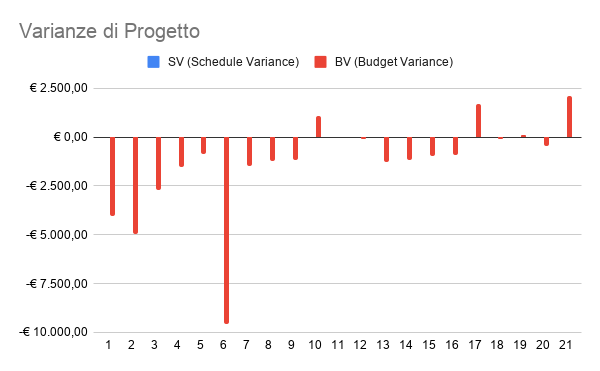
\includegraphics[width=0.8\textwidth]{grafici/varianze.png}
	    \caption{Andamento SV\textsubscript{G}, BV\textsubscript{G}}
	 \end{figure}

Il grafico illustra l'andamento della Schedule Variance\textsubscript{G} (SV) e della Budget Variance\textsubscript{G} (BV).

Coerentemente con quanto osservato nei trend di progetto, la Schedule Variance si mantiene costantemente a 0,00~\euro\ per tutti i 21 sprint: questo è il risultato matematico del perfetto allineamento tra il lavoro completato (EV) e quello pianificato (PV), confermando la totale assenza di ritardi temporali.

Per quanto riguarda la Budget Variance, dopo il marcato avanzo positivo registrato negli sprint 9 e 10, negli sprint 13 e 14 si evidenziano lievi variazioni negative (pari rispettivamente a -19,17~\euro\ nello sprint 13 e -12,50~\euro\ nello sprint 14). Successivamente, la varianza cumulata si attesta a -71,60~\euro\ nello Sprint 18, con un lieve scostamento negativo nel singolo sprint (pari a -3,33~\euro) rispetto al forte consolidamento positivo registrato nello Sprint 17. Successivamente negli sprint dal 19 e 20 si ha una stabilizzazione vicino allo 0 con solo un leggero picco nello sprint 21. Tali scostamenti, dovuti al maggior carico orario richiesto dai ruoli di Amministratore e Verificatore, rientrano ampiamente nelle soglie di tolleranza ammissibili e non compromettono la stabilità economica del progetto, che registra un totale di risorse residue solido per la fase di Product Baseline.


\subsubsection{Indici di Performance}
 \begin{figure}[H]
	    \centering
	    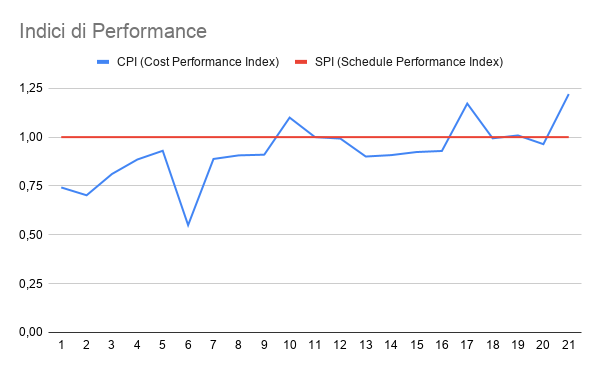
\includegraphics[width=0.8\textwidth]{grafici/performance.png}
	    \caption{Andamento CPI, SPI}
	 \end{figure}

Il grafico riporta l'andamento sprint per sprint del Cost Performance Index (CPI) e dello Schedule Performance Index (SPI). 

Lo SPI si mantiene stabilmente sulla linea ottimale di 1,0 per tutti i 21 sprint conclusi, a dimostrazione di una pianificazione e di un'esecuzione delle tempistiche costantemente prive di ritardi.

Il CPI, dopo essere risalito sopra la soglia ottimale di 1,0 negli sprint 9, 10 e 11, nelle successive iterazioni si è assestato su valori prossimi alla parità (0,90 nello sprint 13 e 0,96 nello sprint 14). Successivamente, dopo un'ulteriore fase di consolidamento, il CPI ha registrato un picco positivo pari a 1,17 nello Sprint 17 per poi assestarsi su un solido 0,99 nello Sprint 18; infine si è tenuto stabile sulla soglia dell' 1,00 con solo un picco nello sprint 21. La combinazione dei due indici (SPI a 1,0 e CPI stabile nell'intorno dell'unità) conferma l'efficienza globale del team sia nel rispetto delle scadenze sia nella gestione oculata del budget allocato in fase operativa.


\subsubsection{Previsione Spesa Finale}
 \begin{figure}[H]
	    \centering
	    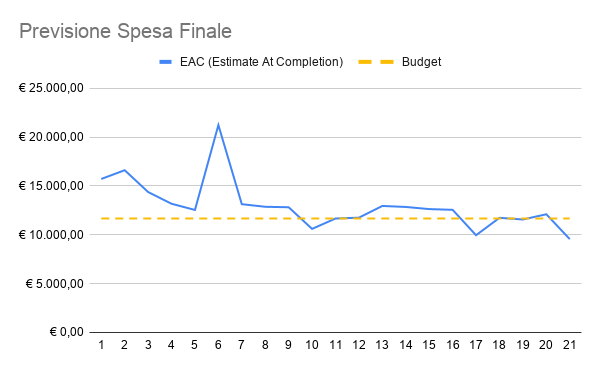
\includegraphics[width=0.8\textwidth]{grafici/previsione_spesa.png}
	    \caption{Andamento EAC\textsubscript{G}}
	 \end{figure}

Il grafico illustra l'andamento dell'Estimate at Completion\textsubscript{G} (EAC). La linea orizzontale tratteggiata rappresenta il BAC\textsubscript{G} (Budget at Completion\textsubscript{G}), fissato a 11.665~\euro.

L'andamento della stima a finire rispecchia l'evoluzione del CPI nel tempo. Superato il picco critico iniziale dello sprint 6 e l'importante fase di recupero culminata negli sprint 9--11, la curva dell'EAC si è inizialmente stabilizzata nelle iterazioni successive al di sotto della linea del BAC, toccando il punto di minimo virtuoso nello Sprint 21 (9.558,31~\euro). Dallo Sprint dal 17 (precedente minimo) in poi fino al 21 l'andamento è stato abbastanza stabile, in corrispondenza del riallineamento delle stime e dell'avvio della codifica.

Tali dati confermano che il gruppo sta mantenendo la proiezione del costo finale complessivo perfettamente in linea con il budget preventivato, garantendo il completamento delle attività entro i limiti finanziari stabiliti.


\subsubsection{Requisiti}
 \begin{figure}[H]
	    \centering
	    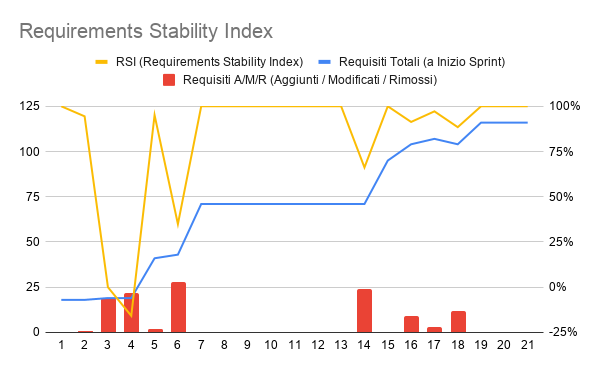
\includegraphics[width=0.8\textwidth]{grafici/RSI.png}
	    \caption{Andamento Requisiti\textsubscript{G}}
	 \end{figure}
Il grafico descrive l'andamento del Requirement Stability Index (RSI) di sprint in sprint.
L'RSI si mantiene stabile nel corso dei vari sprint. Si nota un incremento sostanziale dei requisiti all'inizio degli sprint 5 e 7, in concomitanza con i riscontri ricevuti durante i colloqui con il docente. Negli sprint successivi, compreso lo sprint 14, l'indice ha evidenziato un'elevata stabilità a seguito del colmamento del gap numerico dei requisiti e del completamento delle tabelle di tracciamento fonti-requisiti. Nello Sprint 18 l'indice mostra una leggera flessione (88,46\%) causata da 12 modifiche o integrazioni al set dei 104 requisiti tracciati all'inizio dell'iterazione; successivamente i requisiti rimangono costanti senza modifica fino allo sprint 21. Questo assestamento è una conseguenza naturale e pianificata dell'integrazione di nuovi requisiti di sistema emersi durante la redazione e il consolidamento dell'architettura nella Specifica Tecnica. Il valore rimane comunque ben al di sopra della soglia di accettabilità, confermando che il nucleo dei requisiti principali del progetto è stabile.

\subsubsection{Correttezza Ortografica}
 \begin{figure}[H]
	    \centering
	    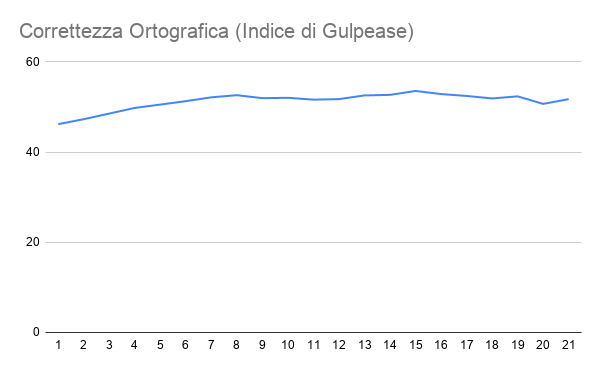
\includegraphics[width=0.8\textwidth]{grafici/gulpease.png}
	    \caption{Indice di Gulpease\textsubscript{G}}
	 \end{figure}
Il grafico illustra l'andamento dell'Indice di Gulpease, utilizzato per monitorare la leggibilità e la chiarezza della documentazione in lingua italiana. 
Nel corso degli sprint si osserva un costante mantenimento di valori compresi nella fascia di accettabilità ($\ge 40$ e $< 80$). Il trend si conferma stabile anche negli ultimi sprint, assestandosi nello Sprint 21 al valore di 51,74. Tale risultato dimostra un livello di leggibilità adeguato e una costante attenzione del gruppo alle attività di revisione editoriale dei documenti, risultato non banale vista la forte introduzione di terminologia tecnica complessa legata all'architettura software.

\subsubsection{Sprint Goal Achievement}
 \begin{figure}[H]
	    \centering
	    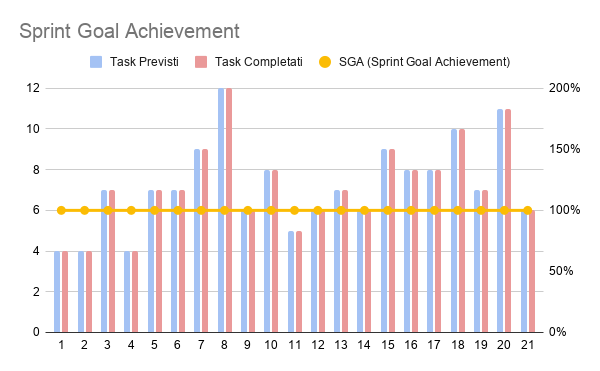
\includegraphics[width=0.8\textwidth]{grafici/task.png}
	    \caption{Andamento task\textsubscript{G}}
	 \end{figure}
Il grafico mostra lo Sprint Goal Achievement (SGA) per osservare il numero di task previste ed effettivamente completate durante i vari sprint. In tutti i 21 sprint svolti finora è stato raggiunto il 100\% di completamento dei task pianificati, confermando la continuità operativa del gruppo e il pieno raggiungimento degli obiettivi stabiliti per ciascun iterazione.